
\subsection{Cloud Service}\label{subsec:cloud-service}

\subsubsection{Architektur}

Es gibt deren Domänen 2. Configuration und Notification.

So quasi als ob man 2 Microservices haben kann. Aber wär halt doof das für den stand jetzt schon so zu trennen, deshalb vorerst mal erst ein einzelnes.

\clearpage

\subsubsection{Domänenmodell}


Für die beiden Domänen gibt es natürlich auch so n paar Diagramme. Die gibts jetzt hier:


\subsubsection*{Domäne Configuration}

\begin{figure}[h]
    \centering
    \begin{minipage}[b]{1.0\textwidth}
        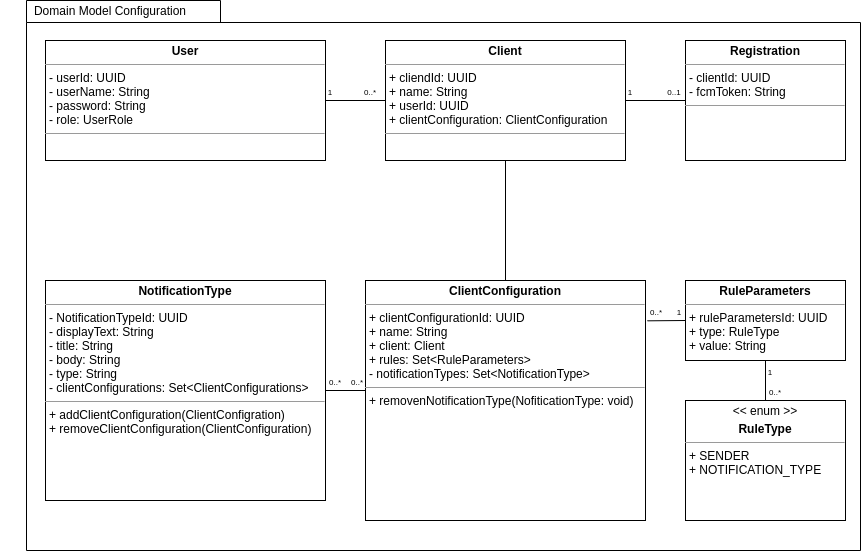
\includegraphics[width=\textwidth]{graphics/Class_Configuration_Domain}
        \caption{Domänenmodell Configuration}
    \end{minipage}
\end{figure}
Also erstmal gibts da son halb generischen konfigurationsmodel.
Wär auch fast mandantenfähig.
Aber halt nur fast.



\clearpage

\begin{figure}[h]
    \centering
    \begin{minipage}[b]{1.0\textwidth}
        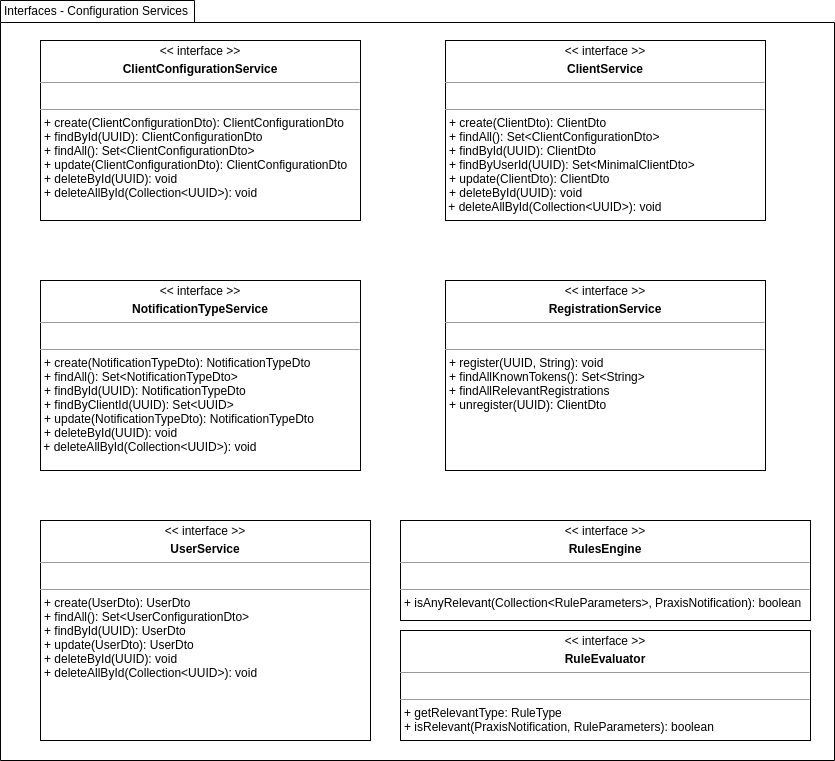
\includegraphics[width=\textwidth]{graphics/Class_Configuration_Services}
        \caption{Klassendiagramm Configuration Service Interfaces}
    \end{minipage}
\end{figure}
Services mit CRUD gibts hier.
Pro Service genau eine Instanz mit Default Prefix.
RulesEngine integration ist hier.
Details see Rules Engine.
Die RulesEngine sowie die RuleEvalautor Services werden ausschliesslich innerhalb der Applikation verwendet und sind nicht über die API zugreifbar.
Alle anderen Services bieten ihre Methoden über eine REST API an. Es wird darauf verzichtet, dass alles nochmal hier zu kopieren.
URL Konzept im Kapitel API.


\clearpage
Dann muss man ja noch sachen darauf auswerten können und zeug.
Das Bild zeigt: Strategy Pattern mit Spring is noch nice.

\begin{figure}[h]
    \centering
    \begin{minipage}[b]{1.0\textwidth}
        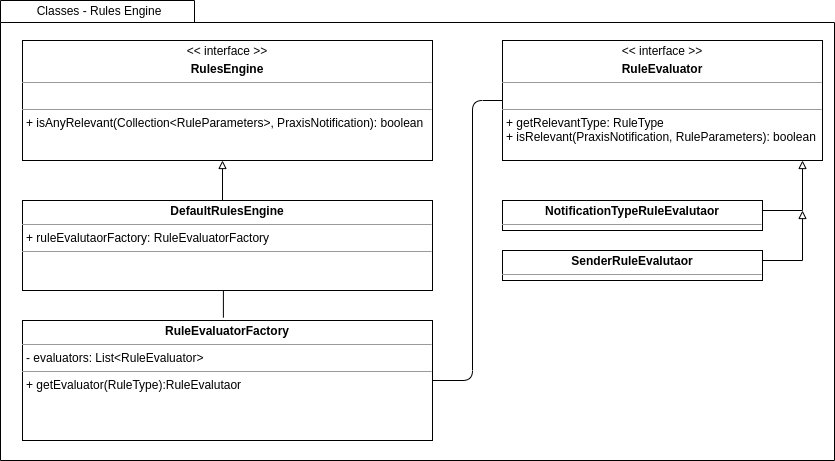
\includegraphics[width=\textwidth]{graphics/Class_Configuration_RulesEngine}
        \caption{Klassendiagramm Rules Engine}
    \end{minipage}
\end{figure}

\clearpage
\subsubsection*{Domäne Notification}

Joa, und die Notifikationen selbst muss ja auch noch wer verschicken.

\begin{figure}[h]
    \centering
    \begin{minipage}[b]{1.0\textwidth}
        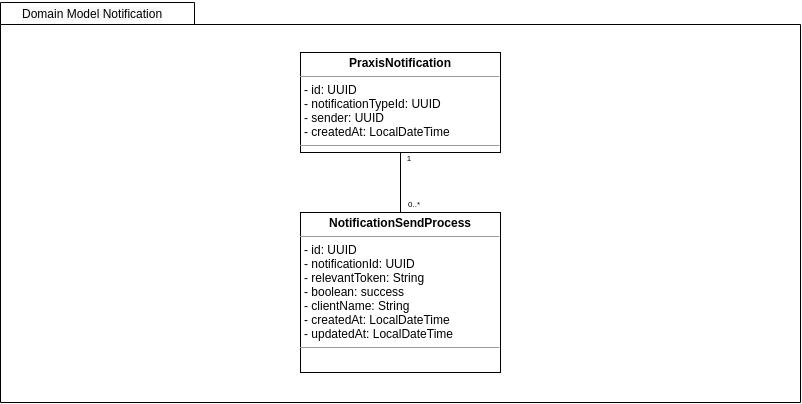
\includegraphics[width=\textwidth]{graphics/Class_Notification_Domain}
        \caption{Domänenmodell Notification}
    \end{minipage}
\end{figure}

Damit man weiss was passiert und teil Zeuch wiederholt werden kann.
Braucht dann klar auch noch n paar Services.




\clearpage

\clearpage
\subsubsection{Laufzeitmodell}

Im Folgenden werden die Abläufe für das Versenden und Empfangen von Benachrichtigungen im Detail definiert.

\subsubsection*{Client Registration}

Pre-Condition: Gültige Konfiguration für Benutzer und Client sind erfasst.

In einem ersten Schritt muss sich der Praxismitarbeiter am Mobile Client anmelden.
Hat er gültige Benutzerdaten angegeben, werden Informationen zu allen verfügbaren Konfigurationen vom Cloud Service geladen und der Benutzer kann die gewünschte Konfiguration auswählen.
Dabei werden nur Name und Id der Konfigurationen geladen, damit nicht mehr Daten als nötig übertragen werden.
Sobald eine Konfiguration ausgewählt ist, werden alle dafür Konfigurierten NotificationTypes geladen und im UI die entsprechenden Buttons erstellt.
Sobald eine Konfiguration geladen ist, registriert sich der Mobile Client beim Messageing Service.
Als Antwort erhält er ein eindeutiges Token, welches verwendet werden kann, um an diesem Client Nachrichten zu senden.
Der Mobile Client Registriert sich schliesslich mit dem Token vom Messaging Service und der ausgewählten Konfiguration beim Cloud Service.
In diesem Zustand ist der Client dem Messaging Service und dem Cloud Service bekannt und ist bereit Benachrichtigungen zu empfangen.

\begin{figure}[h]
    \centering
    \begin{minipage}[b]{1.0\textwidth}
        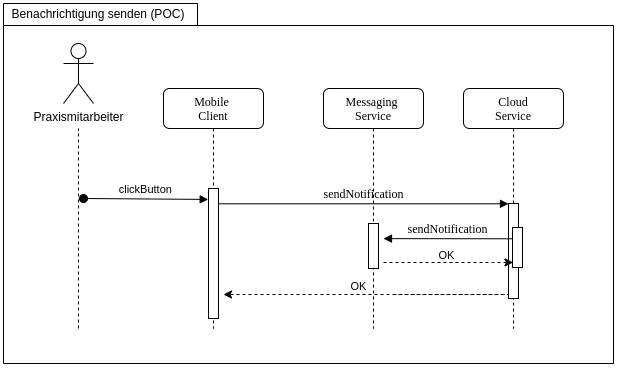
\includegraphics[width=\textwidth]{graphics/Sequence_POC_Send}
        \caption{Ablauf Client Registrierung}
    \end{minipage}
\end{figure}


\subsubsection*{Benachrichtigung versenden und empfangen}

Pre-Condition: Client Registrierung ist für 2 Clients abgeschlossen. Es bestehen gültige Subscriber Configs. Konfiguration ist geladen.

Der Benutzer tippt auf einen der Benachrichtigungsbuttons.
Pro Button ist die Id des verbundenen NotificationTypes hinterlegt.
Es wird nun eine Anfrage an den NotificationController im Cloud Service gesendet.
Darin enthalten sind die Id des Absender Clients und die Id des NotificationTypes.
Der NotificationController macht eine Anfrage an den ConfigurationController um alle relevanten empfänger zu finden.
Im ConfigurationController werden alle konfigurierten ClientConfigurations nach Subscriber Regeln evaluiert.
Der ConfigurationController gibt schliesslich eine Liste der Registrations zurück die zu einer ClientConfiguration gehören für die eine der Konfigurierten Regeln zugetroffen hat.
Der NotificationController lädt den NotificationType aus der Send-Anfrage und benutzt diese Daten um eine Benachrichtigung an alle Empfänger für die er gerade Registrations geladen hat zu senden.
Der NotificationController meldet zurück, ob der Versand an alle Empfänger funktioniert hat.
Ist dies nicht der Fall wird der Retry-Process auf Client Seite gestartet.

\begin{figure}[h]
    \centering
    \begin{minipage}[b]{1.0\textwidth}
        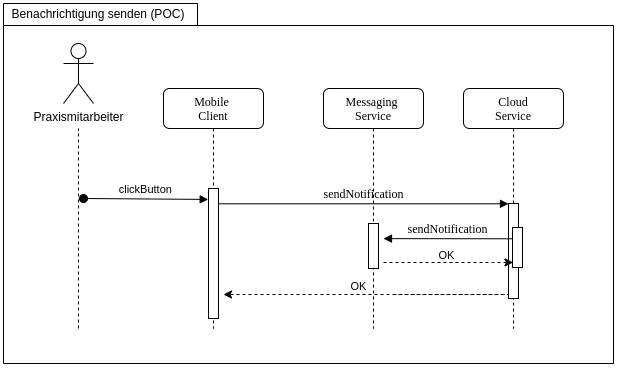
\includegraphics[width=\textwidth]{graphics/Sequence_POC_Send}
        \caption{Ablauf Client Registrierung}
    \end{minipage}
\end{figure}


\subsubsection*{Benachrichtigung wiederholen}

Pre-Condition: Benachrichtigung versendet und mind. 1 Versand fehlgeschlagen.

Der Client zeigt einen Dialog an in dem der Benutzer informiert wird und gefragt wird, ob er die Fehlgeschlagenen wiederholen möchte.
Bestätigt der Benutzer wird eine Retry-Anfrage an den NotificationController gesendet.
Parameter ist die technische id der Notification die fehlgeschlagen ist.
NotificationController durchsucht die NotificationSendProcess tabelle nach der gegebenen id und filtert auf fehlgeschlagene.
Anschliessend wird der send prozess anhand der tokens in dieser NotificationSendProcess Instanzen wiederholt.


\clearpage

\subsubsection{API}

S gibt da n paar controller und die brauchen ein paar services.
